\documentclass[times,utf8,diplomski]{fer}
\usepackage{booktabs}
\usepackage{tabularx}
\usepackage{listings}
\usepackage{amsmath}
\usepackage{graphicx}
\usepackage{algorithmic}
\usepackage{algorithm2e}
\usepackage{cancel}
\usepackage{listings}
\usepackage{caption}



\begin{document}

\thesisnumber{2149}

\title{Inverzna kinematika manipulatora ostvarena pomoću dubokog potpornog učenja}

\author{Josip Torić}



%%\maketitle

%%%\izvornik

\zahvala{ Zahvaljujem mentorici izv. prof. dr. sc.~Mariji Seder te suradniku mag. ing.~Filipu Mariću na motivaciji i savjetima prilikom pisanja ovog rada.

	Zahvaljujem svojoj majci i svome ocu koji su me uvijek podržavali.

	Zahvaljujem svojoj djevojci Rebeki što je preživjela sa mnom ovu godinu.
}

\tableofcontents

%%%%%%%%%%%%%%%%%%%%%
\chapter{Uvod}

Živimo u svijetu prepunom informacija, zadataka i problema. Ljudi su tijekom godina evoluirali da se uspješno mogu nositi s ovim svijetom. Ono što ljudi sada žele napraviti je da se i roboti mogu nositi s ovim svijetom. Bez brige, nismo ni približno dogurali do točke kada će roboti nas u potpunosti zamijeniti.

Uzmimo samo jednostavan zadatak na primjer kao što je podizanje objekta s poda. Čovjek vidi objekt, ocjeni kako da ga najlakše uhvati i uzme ga u ruku. Kada bismo robota, odnosno računalo željeli projektirati za takav zadatak, ubrzo bismo uvidjeli da to nije tako jednostavna stvar. Objekti dolaze u svakakvim oblicima i težinama, a obične stvari iz programiranja kao što su for-petlje i if-blokovi tu nam neće previše pomoći.

Računalni znanstvenici su nakon Drugog svjetskog rata krenuli razvijati umjetnu inteligenciju. Umjetna inteligencija je naziv koji pridajemo svakom neživom sustavu koji pokazuje sposobnost snalaženja u novim situacijama. Unutar umjetne inteligencije postoje razna područja istraživanja, a jedan od njih je strojno učenje. Strojno učenje je grana umjetne inteligencije koja se bavi oblikovanjem algoritama koji svoju učinkovitost poboljšavaju na temelju empirijskih podataka. Unutar strojnog učenja postoji također mnogo grana, a jedna od njih, ujedno i jedna od najmlađih, je potporno učenje. Potporno učenje se bavi programskim agentima koji rješavaju zadatke koji su stavljeni pred njih metodom pokušaja i pogrešaka. Agent se nalazi u okruženju te u tom okruženju mu stoje na raspolaganju brojne akcije čiji će rezultat biti prelazak u novo stanje i eventualna nagrada. Upravo zbog tog koncepta, potporno učenje je iznimno pogodno u robotici jer roboti se ipak nalaze u realnom svijetu, a ne virtualnom.

Cilj ovog diplomskog rada je naučiti inverznu kinematiku robotske ruke Jaco uz primjenu dubokog potpornog učenja. Iznijet ću teorijske osnove potpornog učenja, praktične primjene potpornog učenja, izvesti algoritam jednostavnog gradijenta politike te dati opis tri algoritma za gradijent politike. Svaki algoritam se nastavlja na prethodni, a finalni algoritam proksimalne optimizacije politike ću iskoristiti za učenje inverzne kinematike robotske ruke Jaco. Problem koji ruka rješava je dohvat loptice u prostoru, prvo bez prepreka te zatim s preprekama. Istraživački dio diplomskog zadatka sastoji se od isprobavanja različitih funkcija nagrade za robotsku ruku koje zatim služe algoritmu potpornog učenje pri treniranju modela.




%%%%%%%%%%%%%%%%%%%
\chapter{Teorijske osnove potpornog učenja}
\section{Osnove potpornog učenja}
\subsection{Koncept potpornog učenja}

Potporno učenje je grana strojnog učenja koja proučava agente i kako oni uče na temelju pokušaja i pogreške. Ono formalizira ideju da nagrađivanje, odnosno kažnjavanje agenta potiče ponavljanje, odnosno izbjegavanje određenog ponašanja u budućnosti.

Potporno učenje je u zadnjih par godina doživjelo uzlet. Korišteno je da bi se računalo naučilo kako kontrolirati robota bilo to u simulaciji, bilo u realnom svijetu, no vjerojatno najpoznatije korištenje potpornog učenja u posljednje vrijeme je bilo stvaranje napredne umjetne inteligencije koja je sposobna igrati strateške igre kao što su šah ili Go ili pak da bude sposobna igrati računalne strateške igre kao što je Dota 2. Umjetna inteligencija koja je proizašla iz ovog potpornog učenja nije samo bila sposobna igrati dotičnu igru, ona je postala najbolja na svijetu u toj igri stvarajući dosad ljudskom umu nezamislive taktike i principe.

Osnovna ideja potpornog učenja je da postoji agent u svojem okruženju. To okruženje može biti bilo što, šahovska ploča, pikseli na ekranu ili pak realni svijet. Agent se u svakom trenutku nalazi u nekom stanju, zatim poduzima neku akciju koja ga odvodi u sljedeće stanje. Ako je došao u dobro stanje, nagradimo ga, a ako je pak došao u loše stanje kaznimo ga. Na temelju toga gradimo politiku odabira akcija agenta. Odabir politike odabira akcija agenta je zapravo potporno učenje \citep{sutton}.

\begin{figure}[ht!]
	\centering
	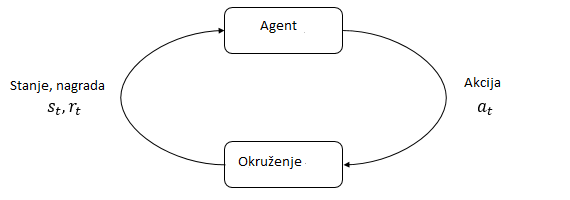
\includegraphics[width=\columnwidth]{img/agent-environment.png}
	\caption{Odnos agent i okruženja.\protect\footnotemark}
	\label{fig:agenta}
\end{figure}
\footnotetext{Preuzeto sa \url{https://spinningup.openai.com}}



\subsection{Duboko potporno učenje}

Politike odabira akcija se spremaju u funkcije. Funkcija na ulaz prima stanje prostora te na izlaz vraća akciju. No, kao i svaka funkcija ona je ograničena s parametrima i klasom funkcija koje pripada. Zbog toga u prošlosti, potporno učenje je imalo limitirane primjene.

Pravi proboj u potpornom učenju se dogodio kada su počeli umjesto funkcije aproksimirati dubokim neuronskim mrežama. Duboka neuronska mreža sastoji se od proizvoljnog broja slojeva koji sadrže proizvoljan broj neurona. Svaki neuron prima ulaze iz neurona prethodnog sloja, nad tim ulazima izračunava neku funkciju sa svojim parametrima i dobiveni rezultat prosljeđuje neuronima sljedećeg sloja. Na prvi neuronski sloj prosljeđujemo ulaze, a sa zadnjeg neuronskog sloja očitavamo izlaze iz neuronske mreže. Ovako koncipirana mreža u stanju je naučiti gotovo sve zamislive funkcije te se pretvoriti u funkcije koje uopće nije moguće opisati matematičkim formulama. Laički govoreći, duboka neuronska mreža ponaša se poput ljudskog mozga.



\section{Osnovni pojmovi potpornog učenja}

Kako bi uspješno razumjeli potporno učenje, potrebno je da razumijemo osnovne pojmove potpornog učenja. \citep{SpinningUp2018}

\subsection{Stanje i opservacija}

Stanje predstavlja kompletan opis trenutnog stanja svijeta. Ne postoji informacija u svijetu koja je skrivena od stanja.

Opservacija predstavlja opis svijeta koje agent vidi. Ako agent je u stanju vidjeti stanje svijeta kroz opservaciju, kažemo da je okruženje viđeno u potpunosti. Ako agent vidi samo dio svijeta, kažemo da je okruženje djelomično viđeno.

U dubokom potpornom učenju gotovo uvijek stanja i opservacije predstavljamo realnim vektorima, matricama ili tenzorima višeg reda. Naprimjer, slika se može predstaviti kao RGB matrica piksela, dok se stanje robota može predstaviti kutevima zglobova ili trenutnom brzinom.

\subsection{Prostor akcija}

Sve dozvoljene akcije u nekom okruženju predstavljaju prostor akcija. Prostor akcija može biti diskretan ili kontinuiran.

Okruženja poput šahovske ploče, igre na starim konzolama poput Atari-a ili ploče za igru Go predstavljaju diskretan prostor akcija. Iz svakog stanja postoji konačan broj akcija koje agent može poduzeti.

Robot u realnom svijetu se nalazi u kontinuiranom prostoru akcija. Iz svakog stanja mu je na raspolaganju beskonačno mnogo akcija koje može poduzeti. U kontinuiranom prostoru akcija, akcije su predstavljene realnim vektorima.

\subsection{Politika}

Politika je pravilo prema kojem agent određuje koju će akciju odabrati. Ona može biti deterministička ili stohastička. Politika je, suštinski govoreći, mozak agenta.

Deterministička politika je uobičajeno označava sa ${\mu}$:

\begin{equation}
	\label{deterministic policy}
	a_t = \mu(s_t)
\end{equation}

\noindent gdje ${a_t}$ označava akciju, a ${s_t}$ stanje svijeta. Stohastička politika se uobičajeno označava sa ${\pi}$:

\begin{equation}
	\label{stochastic policy}
	a_t \sim \pi(\cdot | s_t)
\end{equation}

\noindent gdje ${a_t}$ također označava akciju, a ${s_t}$ stanje svijeta.

U dubokom potpornom učenju politike su parametrizirane s parametrima neuronske mreže i možemo ih trenirati s algoritmima za treniranje neuronske mreže. Parametre najčešće označavamo s ${\theta}$ ili ${\phi}$ te onda možemo pisati:

\begin{equation}
	\label{neural network policy}
	\begin{aligned}
		a_t = \mu_{\theta}(s_t) \\
		a_t \sim \pi_{\theta}(\cdot | s_t)
	\end{aligned}
\end{equation}

\noindent čime označavamo da je politika ovisna o parametrima neuronske mreže.

\subsection{Putanja}

Putanja je slijed stanja i akcija koje se događaju u okruženju.

\begin{equation}
	\label{trajectory}
	\tau = (s_0, a_0, s_1, a_1, ...).
\end{equation}

\noindent gdje ${\tau}$ predstavlja putanju. Početno stanje se uvijek slučajno izabire.

Prijelazi u sljedeće stanje su uvjetovani prirodnim zakonima okruženja i ovise samo o posljednjoj akciji. Prijelazi mogu biti deterministički ili stohastički.


\subsection{Nagrada}

Nagrada predstavlja vrijednost kojom ćemo nagraditi agenta ako poduzme neku akciju u nekom stanju.


\begin{equation}
	\label{reward}
	r_t = R(s_t, a_t, s_{t+1})
\end{equation}

\noindent gdje ${r_t}$ predstavlja vrijednost nagrade, a ${R}$ funkciju nagrade. Ovaj izraz se često pojednostavljuje kao funkcija trenutnog stanja ${r_t = R(s_t)}$ ili funkcija trenutnog stanja i akcije ${r_t = R(s_t,a_t)}$.

Cilj agenta je maksimizirati ukupnu nagradu duž putanje. U maksimiziranju nagrade nailazimo na dva principa, ovisno imamo li konačnu ili beskonačnu putanju. U slučaju konačne putanje dovoljno je samo sumirati sve nagrade duž putanje prema formuli:

\begin{equation}
	\label{finite reward}
	R(\tau) = \sum_{t=0}^T r_t.
\end{equation}

\noindent a kod beskonačne putanje potrebno je nagradu ipak skalirati s faktorom propadanja ${\gamma \in (0,1)}$:

\begin{equation}
	\label{infinite reward}
	R(\tau) = \sum_{t=0}^{\infty} \gamma^t r_t.
\end{equation}

\noindent gdje ${\gamma}$ predstavlja faktor propadanja.

U mnogo problema nemamo nagradu nego kaznu, koju označimo s ${p_t}$. Problem potpornog učenja onda možemo shvatiti kao maksimizator negativne kazne, čime će cilj agenta biti nagradu približiti što moguće bliže nuli.

\begin{equation}
	\label{finite punishment}
	R(\tau) = \sum_{t=0}^T -p_t.
\end{equation}


\subsection{Problem potpornog učenja}

Problem potpornog učenja je odabrati optimalnu politiku koja će maksimizirati očekivanu nagradu kada se agent ponaša u skladu s odabranom politikom. Matematička formulacija tog problema polazi od vjerojatnosti odabira pojedine putanje uz danu politiku koja glasi:
\begin{equation}
	\label{probability trajectory}
	P(\tau|\pi) = \rho_0 (s_0) \prod_{t=0}^{T-1} P(s_{t+1} | s_t, a_t) \pi(a_t | s_t)
\end{equation}

\noindent gdje ${P}$ predstavlja vjerojatnost odabira putanje uz danu politiku. Očekivana ukupna nagrada se onda može iskazati prema formuli:

\begin{equation}
	\label{ukupna nagrada}
	J(\pi) = \int_{\tau} P(\tau|\pi) R(\tau) = \underset{\tau\sim \pi} E[{R(\tau)}]
\end{equation}

\noindent gdje ${J(\pi)}$ predstavlja ukupnu nagradu za danu politiku, a ${\underset{\tau\sim \pi}E}$ putanju s danom politikom. Optimizacijski problem se onda može iskazati kao:

\begin{equation}
	\label{optimizacijski problem}
	\pi^* = \arg \max_{\pi} J(\pi)
\end{equation}

\noindent gdje ${\pi^*}$ predstavlja optimalnu politiku.

\subsection{Funkcije vrijednosti}

U potpornom učenju je često korisno znati vrijednost pojedinog stanja ili stanja i akcije koja slijedi. Vrijednost stanja označava očekivanu nagradu koju dobijemo ako krenemo iz tog stanja i onda uvijek postupamo po nekoj politici.

Postoje 4 glavne vrijednosne funkcije. Prva funkcija glasi:

\begin{equation}
	\label{prva vrijednosna}
	V^{\pi}(s) = \underset{\tau \sim \pi} E [{R(\tau)\left| s_0 = s\right.}]
\end{equation}

\noindent gdje ${V^{\pi}(s)}$ predstavlja vrijednosnu funkciju. Ova funkcija predstavlja očekivanu nagradu ako krenemo iz stanja ${s}$ i uvijek se ponašamo prema politici ${\pi}$.


\begin{equation}
	\label{druga vrijednosna}
	Q^{\pi}(s,a) = \underset{\tau \sim \pi}E[{R(\tau)\left| s_0 = s, a_0 = a\right.}]
\end{equation}

\noindent Ova funkcija predstavlja očekivanu nagradu ako krenemo iz stanja ${s}$, odaberemo akciju ${a}$ i zatim se ponašamo prema politici ${\pi}$.

\begin{equation}
	\label{treća vrijednosna}
	V^*(s) = \max_{\pi} \underset{\tau \sim \pi}E[{R(\tau)\left| s_0 = s\right.}]
\end{equation}

\noindent Ova funkcija predstavlja očekivanu nagradu ako krenemo iz stanja ${s}$ i uvijek se ponašamo prema optimalnoj politici.

\begin{equation}
	\label{četvrta vrijednosna}
	Q^*(s,a) = \max_{\pi} \underset{\tau \sim \pi}E[{R(\tau)\left| s_0 = s, a_0 = a\right.}]
\end{equation}

\noindent Ova funkcija predstavlja očekivanu nagradu ako krenemo iz stanja ${s}$, odaberemo akciju ${a}$ i zatim se ponašamo prema optimalnoj politici.

Iz ovih funkcija se može još definirati i funkcija prednosti koja glasi:

\begin{equation}
	\label{funkcija prednosti}
	A^{\pi}(s,a) = Q^{\pi}(s,a) - V^{\pi}(s)
\end{equation}

\noindent gdje ${A^{\pi}(s,a)}$ predstavlja prednosti za dano stanje i akciju. Ova funkcija nam govori koliko je dana akcija bolja od ostalih akcija u prosjeku.


Ove sve funkcije zadovoljavaju rekurzivne Bellmanove jednadžbe \citep{Bellman716}:

\begin{equation}
	\label{belman 1}
	V^{\pi}(s) = \underset{a \sim \pi \\ s'\sim P}E[{r(s,a) + \gamma V^{\pi}(s')}]
\end{equation}

\begin{equation}
	\label{belman 2}
	Q^{\pi}(s,a) = \underset{s'\sim P}E[{r(s,a) + \gamma \underset{a'\sim \pi}E[{Q^{\pi}(s',a')}}]]
\end{equation}

\begin{equation}
	\label{belman 3}
	V^*(s) = \max_a \underset{s'\sim P}E[{r(s,a) + \gamma V^*(s')}]
\end{equation}

\begin{equation}
	\label{belman 4}
	Q^*(s,a) = \underset{s'\sim P}E[{r(s,a) + \gamma \max_{a'} Q^*(s',a')}]
\end{equation}

\noindent Sve Bellmanove jednadžbe govore istu stvar, a to je da vrijednost početnog stanja se sastoji od nagrade što se nalazimo u tom stanju zbrojena s vrijednosti svih stanja u kojima ćemo se naći u sljedećim koracima.

\section{Podjela algoritama potpornog učenja}

Algoritmi potpornog učenja dijele se na algoritme s modelom i algoritme bez modela. U algoritmima s modelom poznat je model okruženja, dok u algoritmima bez modela nije poznat model okruženja.

Prednost algoritama s modelom je ta što je moguće promatrati više stanja i akcija unaprijed jer se unaprijed zna u kojem će se stanju završiti za pojedinu akciju. Algoritmi s modelom se dijele na algoritme u kojima se pokušava naučiti model svijeta te na one algoritme u kojima je model unaprijed poznat. No, učenje modela je također iznimno težak problem te postoji velika mogućnost da se agent odlično ponaša u naučenom modelu, ali se ponaša loše u stvarnom okruženju jer je pristrano naučio model svijeta. Algoritmi s modelom se odlično ponašaju upravo u slučaju kada model postoji. Najbolji primjer ovoga je algoritam AlphaZero \citep{alphazero} koji je uspio pobijediti svjetskog prvaka u igri Go te postati najbolji računalni program za igranje šaha.

Algoritmi bez modela su prilagođeniji realnom svijetu i kao takvi su više razvijeniji nego algoritmi s modelom. Oni se dijele na algoritme optimizacije politike gdje se pokušava naći optimalna politika te algoritme Q-učenja gdje se pokušava aproksimirati optimalna Q-funkcija.

\begin{figure}[ht!]
	\centering
	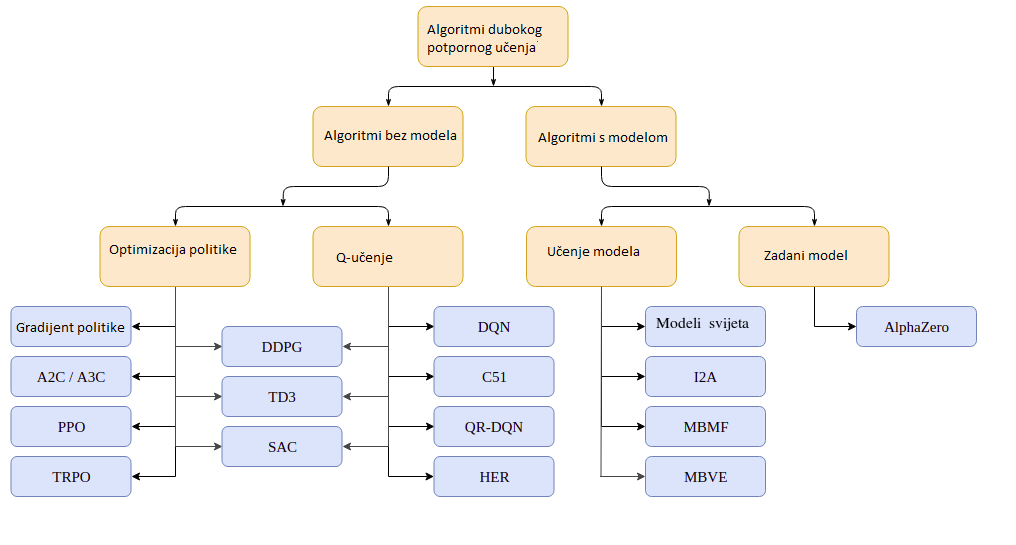
\includegraphics[width=\columnwidth]{img/podjela.png}
	\caption{Podjela algoritama dubokog potpornog učenja.\protect\footnotemark}
	\label{fig:atari}
\end{figure}
\footnotetext{Preuzeto sa \url{https://spinningup.openai.com}}

U ovom diplomskom radu ću se koncentrirati na algoritme bez modela. Model stvarnog svijeta u kojem postoji robotska ruka ili simulator u kojem se nalazi robotska ruka je gotovo nemoguće izgraditi jer se radi o kontinuiranom realnom svijetu. Položaj objekata se mijenja, pod utjecajem je stvarnih sila te kada bi i pokušali izgraditi model stvarnog svijeta on bi bio užasno kompliciran i vjerojatno loše estimirao stvarni svijet. Zbog toga ću koristiti algoritme bez modela i to algoritme optimizacije politike jer su prilagođeniji problemu inverzne kinematike. Algoritmi optimizacije politike direktno optimiziraju cilj koji želimo, dok Q-učenje prvenstvo želi zadovoljiti Bellmanove jednadžbe, a cilj optimizira indirektno.

%%%%%
\chapter{Praktične primjene potpornog učenja}

\section{Primjene u igranju šaha}

Šah je društvena igra za svoje na ploči koja postoji već stotinama godina. Igra se na ploči od 64 polja, a svaki igrač kontrolira 16 figura. Postoji otprilike ${10^{120}}$ mogućih šahovskih partija te iz ovoga vidimo da je nemoguće riješiti problem pobjede u šahu s čistim pretraživanjem prostora.

Većina današnjih računalnih programa za igranje šaha ipak počiva na nekom principu pretraživanja prostora, naravno poboljšanim s raznim heuristikama. Najbolji programi su u stanju pretraživati i do 70 milijuna poteza u sekundi. To je naravno i više nego dovoljno da se pobjedi najbolji svjetski šahovski velemajstor, ali duboko potporno učenje je pokazalo da možemo i bolje igrati šah nego što nam to dozvoljava čista procesorska snaga.

Algoritmi bazirani na dubokom potpornom učenju, kao što su AlphaZero \citep{alphazero} i Leela Chess Zero  \citep{lc0}, uspjeli su kombinirati računalnu snagu s ljudskom intuicijom. Algoritmi su naučeni tako da su im unesena osnovna pravila šaha, dakle poznat im je model svijeta, okruženje i moguće akcije iz svakog stanja. Nakon toga, učenje se obavlja tako da algoritam igra sam protiv sebe i tako poboljšava svoju igru.

Jednom naučen algoritam, koji se naravno poboljšava iz sekunde u sekundu, u stanju je pobijediti apsolutno svakoga, kako čovjeka tako i programe bazirane na pretraživanju stanja. Algoritam ne pretražuje ni približno puno poteza kao program baziran na pretraživanju stanja, on pretražuje naime samo oko 80 tisuća poteza. Međutim, on pretražuje samo poteze koji imaju smisla s obzirom na politiku s kojom je naučen. Na ovaj način, algoritam je uspio potvrditi optimalnost nekih ljudskih ideja u šahu, ali isto tako i odbacio je neke ideje stare stotinu godina. Promatranje algoritama baziranih na potpornom učenju dok igraju šah, omogućava ljudima da poprave vlastitu igru tako što će krenuti razmatrati neke ideje koje su se prije činile besmislene.

\section{Primjene u igranju računalnih igara}

Računalne igre, za razliku od igara na ploči, su korak bliže realnom svijetu. Nemoguće je izraditi model računalne igre, pogotovo u situacijama kada igru igraju više od 2 igrača. Iz ovog razloga, znanstvenicima koji se bave dubokim potpornim učenjem iznimno je zanimljivo vidjeti kako će se algoritmi ponašati u ovim situacijama jer zaključke koje pronađu u ovoj domeni pomoći će im u primjenama u realnom svijetu.

Vjerojatno jedna od najpoznatijih primjena dubokog potpornog učenja u zadnje vrijeme je kada je skupina znanstvenika okupljena u OpenAI timu razvila botove koji su postali bolji od svjetskih prvaka u računalnoj igri Dota 2 \citep{openai2019dota}. Dota 2 je igra koja se igra u 2 tima, a svaki tim čini 5 igrača. Svaki igrač upravlja jednim herojem (u igri trenutno postoji 117 heroja) te je cilj srušiti protivničku bazu. Svaki igrač tijekom same partije, koja traje u prosjeku oko 35 minuta, kupuje razne predmete koji poboljšavaju vlastitog heroja, a novac za predmete zarađuje tako što ubija protivničke heroje ili neutralna čudovišta. Iz ovog jednostavnog opisa same igre, može se vidjeti da je ovo izuzetno težak problem za modelirati uobičajenim računarskim načinima.

Algoritam koji su razvili u OpenAI timu, prima informacije iz same igre 7 puta u jednoj sekundi. Informacije se sastoje od stanja vlastitog tima, stanja protivničkog tima i stanja same mape. Sve ove informacije vidi i stvarni igrač koji igra samu igru, algoritam ne vidi ništa više niti manje. Na temelju tih informacija, algoritam uz pomoć utrenirane politike koja je predstavljena neuronskom mrežom, na izlaz izbacuje akciju koju treba sljedeću poduzeti. Impresivna stvar je ta što ne igra samo jedna instanca algoritma, već igraju 5 instanci koje surađuju.

Slično kao i u robotskim zadacima, algoritmu je zadana funkcija nagrade koja nagrađuje pobjedu protiv drugog time, ubojstvo protivničkog igrača, skupljanje zlatnika i ostale stvari koje su prisutne u samoj igri. Treniranje se odvijalo tako što je igrao igru sam protiv sebe. U prvim epohama, heroji su besmisleno šetali po mapi, nakon prvih par sati počeli su se pojavljivati koncepte koje viđamo u ljudskim partijama, a nakon nekoliko dana algoritam je pokazao i napredne taktike. Nakon 10 mjeseci svakodnevnog treniranja, algoritam je bio u stanju potpuno nadigrati svjetske prvake u ovoj igri i to s taktikama koje su prvi put viđene u 10 godina postojanja ove igre.

Jedan od čestih benchmarkova za evaluiranje rada različitih algoritama dubokog potpornog učenja je igranje igara na konzoli Atari 2600. Konzola Atari 2600 izašla je 1977. godine i doživjela ogromnu popularnost. Razlog zašto se koriste igre na ovoj konzoli je taj što je model same igre najčešće složen te nije optimalno primijeniti algoritme s modelom, opservacija se sastoji od samo 128 piksela, a akcija se sastoji od diskretnih varijabli koje označavaju pomak joysticka ili pritisak na crveni gumb kontrolera. Postoji mnogo različitih igara za Atari konzolu koje su sve ostvarene u emulatoru te je iznimno uspostaviti cjevovod treniranja.

\begin{figure}[ht!]
	\centering
	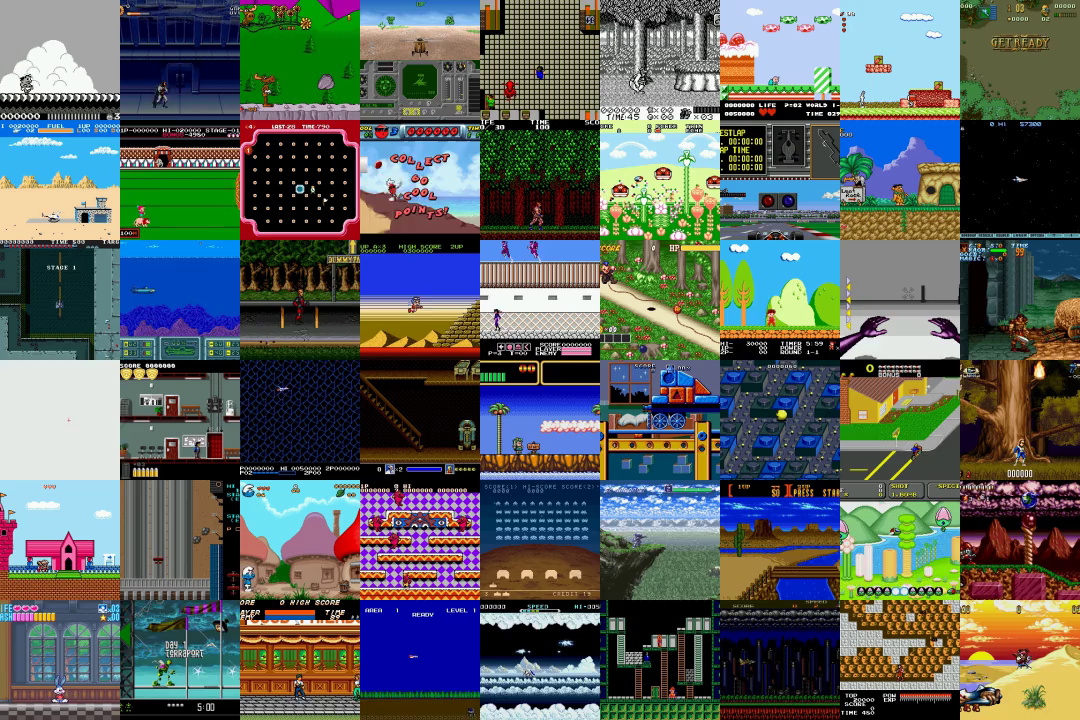
\includegraphics[width=\columnwidth]{img/atari.png}
	\caption{Neke od igara dostupne za Atari 2600.\protect\footnotemark}
	\label{fig:podjela}
\end{figure}
\footnotetext{Preuzeto sa \url{https://openai.com}}

\section{Primjene u robotici}

Robotika je sigurno najzanimljivije i najkorisnije područje primjene dubokog potpornog učenja jer kod robota okruženje je stvarni svijet i njihove akcije imaju posljedice u stvarnom svijetu. No, zbog prirode svijeta i fizičkih zakona koji ovdje vladaju, ovo područje je definitivno i najkompliciranije.

Robotu su najčešće dostupne informacije o položaju u kojem se nalazi, zatim o kutevima zglobova koji ga pokreću, trenutnoj brzini, brzini zglobova, preprekama u prostoru, itd. Na temelju tih informacija, uz pomoć istrenirane politike, određuje koja će mu biti sljedeća akcija. Jedan od najvećih problema vezano za robotiku je nepraktičnost treniranja robota. U stvarnom svijetu je gotovo nemoguće trenirati algoritam zbog ograničenih resursa te jedina mogućnost postaje simulator kojeg nije uvijek baš lako izraditi  \citep{kalas}.

Glavni zadatak ovog diplomskog rada je naučiti inverznu kinematiku robotske ruke Jaco prilikom dohvaćanja loptice iz okruženja, prvo bez prepreka te zatim s preprekama. Robotska ruka je fiksirana te ima informaciju o trenutnom položaju vrha ruke, položaju loptice i položaju prepreka. Robot ima 6 zglobova koji pomiču robotsku ruku, a robotom se upravlja tako da mu se zadaju brzine tih zglobova.

%%%%%%%%%%%%%%%%%%%

\chapter{Algoritmi optimizacije politike}

\section{Pregled algoritama optimizacije politike}

Najosnovniji algoritam optimizacije politike je algoritam jednostavnog gradijenta politike. No, problem kod njega je prevelika nestabilnost. Zbog toga ću iznijeti još dva algoritma, algoritam optimizacije politike uz regije povjerenja i algoritam proksimalne optimizacije politike. Oba algoritma imaju sličnu ideju, poboljšati politiku iz iteracije u iteraciju bez da se previše udalje od prethodne politike. Preveliko udaljavanje od prethodne politike je upravo ono što uzrokuje preveliku nestabilnost kao algoritma jednostavnog gradijenta.

\section{Izvod jednostavnog gradijenta politike}

Osnova za algoritme gradijenta politike je izvod gradijenta politike \citep{schulman}. Gradijent se može izvesti na sljedeći način:

\begin{align*}
	\label{izvod}
	 & \nabla_{\theta} J(\pi_{\theta}) = \nabla_{\theta} \underset{\tau \sim \pi_{\theta}}E[{R(\tau)}]                                                           &                                            \\
	 & = \nabla_{\theta} \int_{\tau} P(\tau|\theta) R(\tau)                                                                                                      & \text{Proširimo očekivanje}                \\
	 & = \int_{\tau} \nabla_{\theta} P(\tau|\theta) R(\tau)                                                                                                      & \text{Dovedimo gradijent unutar integrala} \\
	 & = \int_{\tau} P(\tau|\theta) \nabla_{\theta} \log P(\tau|\theta) R(\tau)                                                                                  & \text{Logaritamski trik}                   \\
	 & = \underset{\tau \sim \pi_{\theta}}E[{\nabla_{\theta} \log P(\tau|\theta) R(\tau)}]                                                                       & \text{Vraćanje u očekivanje}               \\
	 & = \underset{\tau \sim \pi_{\theta}}E[{\nabla_{\theta} (\log \rho_0 (s_0) + \sum_{t=0}^{T} ( \log P(s_{t+1}|s_t, a_t)}]  +                                                                              \\
	 & \underset{\tau \sim \pi_{\theta}}E[{\log \pi_{\theta}(a_t |s_t))) R(\tau)}]                                                                               & \text{Proširimo log-vjerojatnost putanje}  \\
	 & = \underset{\tau \sim \pi_{\theta}}E[{( \cancel{\nabla_{\theta}\log \rho_0 (s_0)} + \sum_{t=0}^{T} ( \cancel{\nabla_{\theta}\log P(s_{t+1}|s_t, a_t)}}] +                                              \\
	 & \underset{\tau \sim \pi_{\theta}}E[{\nabla_{\theta}\log \pi_{\theta}(a_t |s_t)) R(\tau)}]                                                                 & \text{Dovedimo gradijent}                  \\
	 & \therefore \nabla_{\theta} J(\pi_{\theta}) = \underset{\tau \sim \pi_{\theta}}E[{\sum_{t=0}^{T} \nabla_{\theta} \log \pi_{\theta}(a_t |s_t) R(\tau)}]     & \text{Gradijent putanje}
\end{align*}

\noindent gdje ${\nabla}$ označava gradijent. Ovo je očekivanje, što znači da ga možemo estimirati s prosjekom uzorka. Skupimo putanje iz okoline, za svaku pronađemo gradijent te uzmemo aritmetičku sredinu svih uzoraka.

\begin{equation}
	\label{aritmeticka svih uzoraka}
	\hat{g} = \frac{1}{|\mathcal{D}|} \sum_{\tau \in \mathcal{D}} \sum_{t=0}^{T} \nabla_{\theta} \log \pi_{\theta}(a_t |s_t) R(\tau),
\end{equation}

\noindent gdje ${\mathcal{D}}$ skup trajektorija. Moguće je pokazati da se funkcija nagrade može zamijeniti i s funkcijom prednosti.


\section{Algoritam jednostavnog gradijenta politike}

Algoritam jednostavnog gradijenta politike je osnovni algoritam dubokog potpornog učenja. On izravno koristi izvod gradijenta politike, samo što umjesto funkcije nagrade koristi funkciju prednosti.

Pseudokod algoritma je sljedeći:

\begin{algorithm}[H]
	\caption{Algoritam jednostavnog gradijenta politike}
	\label{vpg}
	\begin{algorithmic}[1]
		\STATE Ulaz:  Inicijalni parametri politike $\theta_0$, inicijalni parametri funkcije vrijednosti $\phi_0$
		\FOR{$k = 0,1,2,...$}
		\STATE Prikupimo listu putanja ${\mathcal D}_k = \{\tau_i\}$ prateći politiku $\pi_k = \pi(\theta_k)$ u okruženju.
		\STATE Izračunajmo nagrade $\hat{R}_t$.
		\STATE Izračunajmo funkciju prednosti $\hat{A}_t$ koristeći trenutnu funkciju vrijednosti $V_{\phi_k}$.
		\STATE Izračunajmo gradijent prema formuli:
		\begin{equation*}
			\hat{g}_k = \frac{1}{|{\mathcal D}_k|} \sum_{\tau \in {\mathcal D}_k} \sum_{t=0}^T \left. \nabla_{\theta} \log\pi_{\theta}(a_t|s_t)\right|_{\theta_k} \hat{A}_t.
		\end{equation*}
		\STATE Izračunajmo nove parametre uz pomoć gradijentnog spusta:
		\begin{equation*}
			\theta_{k+1} = \theta_k + \alpha_k \hat{g}_k,
		\end{equation*}
		\STATE Izračunajmo nove parametre funkcije vrijednosti
		\begin{equation*}
			\phi_{k+1} = \arg \min_{\phi} \frac{1}{|{\mathcal D}_k| T} \sum_{\tau \in {\mathcal D}_k} \sum_{t=0}^T\left( V_{\phi} (s_t) - \hat{R}_t \right)^2,
		\end{equation*}
		\ENDFOR
	\end{algorithmic}
\end{algorithm}

\bigskip

Algoritam koristi dvije neuronske mreže. Jedna se koristi za funkciju politike, ona na ulaz prima opservaciju, a na izlaz šalje akciju, a druga se koristi za funkciju vrijednosti koja na ulaz prima opservaciju, a na izlaz šalje broj koji predstavlja vrijednost funkcije. Ako ćemo biti precizniji, neuronska mreža za politiku na izlaz šalje vjerojatnosti poduzimanja pojedinih akcija iz kojih onda algoritam odabire akciju koju će poduzeti te je zbog toga ona stohastička politika. Ovo je bitno zbog računanja funkcije prednosti koja predstavlja razliku između nagrade pridobivene s putanjom kroz okruženje i nagrade koju nam je vratila funkcija vrijednosti. U prijevodu, funkcija prednosti nam govori koliko je akcija koju smo poduzeli bolja od akcije koju bi najčešće poduzeli.

Ako sad bolje pogledamo sada funkciju pogreške, možemo shvatiti što ona zapravo radi. Ako je akcija bila bolja nego prosječna akcija, povećat ćemo vjerojatnost da u budućnosti opet napravimo tu akciju, a ako je akcija bila lošija nego prosječna akcija, smanjit ćemo vjerojatnost da u budućnosti opet napravimo tu akciju. Ovaj algoritam iako jednostavan, predstavlja osnovu svih algoritama dubokog potpornog učenja \citep{schulman}.

\section{Algoritam optimizacije politike uz regije povjerenja}

Problem koji nastaje pri algoritmu jednostavnog gradijenta politike je prevelika nestabilnost. Razlog tome je što nitko ne brani modelu da radikalno promjeni politiku iz koraka u korak. U početnim koracima algoritma, model se ponaša prilično nasumično te ima puno politika koje su bolje od trenutačne iako su sigurno suboptimalne. No, kako se prikupljanje i treniranje podataka događa istodobno, imamo situaciju ako odemo u suboptimalnu politiku, prikupljeni podatci će nam također biti suboptimalni, a to će rezultirati tome da ćemo jako sporo ili nikako doći do globalnog optimuma politike. Ovaj problem se rješava tako da ograničimo algoritmu koliko smije u pojedinom koraku promijeniti politiku. Način na koji je ostvareno u algoritmu optimizacije politike uz regije povjerenja \citep{trpo} je da ograničimo Kullback-Leiblerovu udaljenost između trenutne i sljedeće politike. Kullback-Leiblerova udaljenost se računa na sljedeći način:

\begin{equation}
	\label{Kullback - Leibler}
	D_\text{KL}(P \parallel Q) = \sum_{x\in\mathcal{X}} P(x) \log\left(\frac{P(x)}{Q(x)}\right),
\end{equation}

\noindent gdje ${P(x)}$ predstavlja jednu politiku, a ${Q(x)}$ drugu politiku. Funkcija gubitka ovog algoritma je definirana u obliku:

\begin{equation}
	\label{TRPO loss}
	{\mathcal L}(\theta_k, \theta) = \underset{s,a \sim \pi_{\theta_k}}E[\frac{\pi_{\theta}(a|s)}{\pi_{\theta_k}(a|s)} A^{\pi_{\theta_k}}(s,a)],
\end{equation}

\noindent uz ograničenje da Kullback-Leiblerova udaljenost ne smije biti veća od zadanog hiperparametra ${\delta}$. U ovoj funkciji gradijent logaritma politike je zamijenjen s kvocijentom između stare i nove politike, a matematički je moguće dokazati da je to identična stvar za problem optimizacije politike. Rješenje ovog sustava se dobije uz pomoć Lagrangeove dualne metode i ono glasi:

\begin{equation}
	\label{TRPO rješenje}
	\theta_{k+1} = \theta_k + \alpha^j \sqrt{\frac{2 \delta}{g^T H^{-1} g}} H^{-1} g,
\end{equation}

\noindent gdje je ${g}$ gradijent trenutne politike izračunat iz podataka prikupljenim novom politikom, ${H}$ Hesseova matrica trenutne politike izračunata iz podataka prikupljenih novom politikom, ${\alpha}$ broj između 0 ili 1, a ${j}$ najmanji nenegativni broj koji će osigurati da Kullback-Leiblerova udaljenost bude zadovoljena. Problem koji se nameće u ovome je računanje inverza Hesseove matrice za matrice koje mogu imati veliki broj parametara. Algoritam rješava ovaj problem tako da izračuna vrijednost ${x = H^{-1}g}$ uz pomoć metode konjugatnog gradijenta. Pseudokod algoritma je sljedeći:


\begin{algorithm}[H]
	\caption{Algoritam optimizacije politike uz regije povjerenja}
	\label{trpo}
	\begin{algorithmic}[1]
		\STATE Ulaz:  Inicijalni parametri politike $\theta_0$, inicijalni parametri funkcije vrijednosti $\phi_0$
		\STATE Hiperparametri: Limit KL udaljenosti, koeficijent traženja unazad ${\alpha}$, maksimalan broj koraka traženja unazad K
		\FOR{$k = 0,1,2,...$}
		\STATE Prikupimo listu putanja ${\mathcal D}_k = \{\tau_i\}$ prateći politiku $\pi_k = \pi(\theta_k)$ u okruženju.
		\STATE Izračunajmo nagrade $\hat{R}_t$.
		\STATE Izračunajmo funkciju prednosti $\hat{A}_t$ koristeći trenutnu funkciju vrijednosti $V_{\phi_k}$.
		\STATE Izračunajmo gradijent prema formuli:
		\begin{equation*}
			\hat{g}_k = \frac{1}{|{\mathcal D}_k|} \sum_{\tau \in {\mathcal D}_k} \sum_{t=0}^T \left. \nabla_{\theta} \log\pi_{\theta}(a_t|s_t)\right|_{\theta_k} \hat{A}_t.
		\end{equation*}
		\STATE Uz pomoć algoritma konjugatnog gradijenta izračunajmo:
		\begin{equation*}
			\hat{x} \approx \hat{H}_k^{-1}\hat{g}_k
		\end{equation*}
		\STATE Izračunajmo nove parametre uz pomoć pretrage unatrag
		\begin{equation*}
			\theta_{k+1} = \theta_k + \alpha^j \sqrt{\frac{2 \delta}{\hat{x}_k^T \hat{H}_k \hat{x}_k}} \hat{x}_k
		\end{equation*}
		\STATE Izračunajmo nove parametre funkcije vrijednosti
		\begin{equation*}
			\phi_{k+1} = \arg \min_{\phi} \frac{1}{|{\mathcal D}_k| T} \sum_{\tau \in {\mathcal D}_k} \sum_{t=0}^T\left( V_{\phi} (s_t) - \hat{R}_t \right)^2
		\end{equation*}
		\ENDFOR
	\end{algorithmic}
\end{algorithm}

\bigskip

\section{Algoritam proksimalne optimizacije politike}

Algoritam proksimalne optimizacije politike \citep{ppo} je motiviran istim problemom kao i algoritam optimizacije politike uz regije povjerenja, a to je koliko najveći korak možemo napraviti pri optimizacije politike bez da slučajno napravimo preveliki korak. Algoritam optimizacije politike uz regije povjerenja to rješava tako da uvodi ograničenje Kullback-Leiblerove udaljenosti, ali uvođenje tog ograničenja prilično komplicira funkciju pogreške i algoritam.

Algoritam proksimalne optimizacije politike taj problem rješava bez uvođenja ograničenja, već ugrađuje ograničenje u funkciju pogreške. Algoritam se oslanja na podrezivanje funkcije gubitka tako da ne pogura politiku previše daleko od prethodne politike.

Funkcija pogreške definirana je na sljedeći način:

\begin{equation}
	\label{PPO loss}
	\resizebox{0.99\hsize}{!}{$L(s,a,\theta_k,\theta) = \min\left(
			\frac{\pi_{\theta}(a|s)}{\pi_{\theta_k}(a|s)}  A^{\pi_{\theta_k}}(s,a), \;\;
			\text{clip}\left(\frac{\pi_{\theta}(a|s)}{\pi_{\theta_k}(a|s)}, 1 - \epsilon, 1+\epsilon \right) A^{\pi_{\theta_k}}(s,a)
			\right),$}
\end{equation}

\noindent gdje ${clip}$ označava funkciju podrezivanja. Ono što ovaj naizgled komplicirani izraz radi, vrlo se jednostavno može objasniti ako ga razdvojimo u dva slučaja, kad je funkcija prednosti pozitivna i kad je negativna. Kad je funkcija prednosti pozitivna, odnosno nova politika je bolja od prethodne, želimo da se pomaknemo u smjeru nove politike, ali opet ne želimo previše da se pomaknemo. Pomaknut ćemo se u smjeru nove politike prema izrazu:

\begin{equation}
	\label{PPO adv gain}
	\min\left(
	\frac{\pi_{\theta}(a|s)}{\pi_{\theta_k}(a|s)}, (1 + \epsilon)
	\right),
\end{equation}

\noindent dakle koliko god nova politika razmjerno udaljenija od prethodne, ali maksimalno ${1+\epsilon}$. Ako je funkcija prednosti negativna, odnosno nova politika je lošija od prethodne, pomaknut ćemo u suprotnom smjeru. Pomaknut ćemo se prema izrazu


\begin{equation}
	\label{PPO adv loss}
	\min\left(
	\frac{\pi_{\theta}(a|s)}{\pi_{\theta_k}(a|s)}, (1 - \epsilon)
	\right),
\end{equation}

\noindent dakle vjerojatnost odabira akcija nove politike će se smanjiti u budućnosti, ali opet ne previše.

Pseudokod algoritma je sljedeći:

\begin{algorithm}[H]
	\caption{Algoritam proksimalne optimizacije politike}
	\label{ppo2}
	\begin{algorithmic}[1]
		\STATE Ulaz:  Inicijalni parametri politike $\theta_0$, inicijalni parametri funkcije vrijednosti $\phi_0$
		\FOR{$k = 0,1,2,...$}
		\STATE Prikupimo listu putanja ${\mathcal D}_k = \{\tau_i\}$ prateći politiku $\pi_k = \pi(\theta_k)$ u okruženju.
		\STATE Izračunajmo nagrade $\hat{R}_t$.
		\STATE Izračunajmo funkciju prednosti $\hat{A}_t$ koristeći trenutnu funkciju vrijednosti $V_{\phi_k}$.
		\STATE Izračunajmo nove parametre politike
		\begin{equation*}
			\phi_{k+1} = \arg \min_{\phi} \frac{1}{|{\mathcal D}_k| T} \sum_{\tau \in {\mathcal D}_k} \sum_{t=0}^T L(s,a,\theta_k,\theta),
		\end{equation*}

		\noindent gdje je
		\begin{equation*}
			\resizebox{0.99\hsize}{!}{$L(s,a,\theta_k,\theta) = \min\left(
					\frac{\pi_{\theta}(a|s)}{\pi_{\theta_k}(a|s)}  A^{\pi_{\theta_k}}(s,a), \;\;
					\text{clip}\left(\frac{\pi_{\theta}(a|s)}{\pi_{\theta_k}(a|s)}, 1 - \epsilon, 1+\epsilon \right) A^{\pi_{\theta_k}}(s,a)
					\right),$}
		\end{equation*}

		\STATE Izračunajmo nove parametre funkcije vrijednosti
		\begin{equation*}
			\phi_{k+1} = \arg \min_{\phi} \frac{1}{|{\mathcal D}_k| T} \sum_{\tau \in {\mathcal D}_k} \sum_{t=0}^T\left( V_{\phi} (s_t) - \hat{R}_t \right)^2
		\end{equation*}
		\ENDFOR
	\end{algorithmic}
\end{algorithm}

\bigskip

Upravo ovaj algoritam ću koristiti pri učenju inverzne kinematike robotske ruke Jaco. Algoritam je trenutno jedan od najbolji koji postoje u dubokom potpornom učenju, varijanta ovog algoritma je korištena za učenje igranja igre "Dota 2" te algoritam u većini robotičkih problema pokazuje veoma dobro ponašanje.

\clearpage
\chapter{Inverzna kinematika robotske ruke Jaco}
\section{Robotski manipulatori}

Robotski manipulatori se sastoje od čvrstih tijela koji su međusobno povezani zglobovima. \citep{robotics} Čvrsta tijela se još nazivaju i članci. Mnogi robotski manipulatori su napravljeni po uzoru na ljudske ruke i noge, gdje članci predstavljaju kosti, a zglobovi ljudske zglobove. Ako između bilo kojeg dva para članaka postoji samo jedan redoslijed zglobova i članaka, govorimo o manipulatoru s otvorenim kinematičkim lancem, inače govorimo o manipulatoru sa zatvorenim kinematičkim lancem. Svaki zglob predstavlja jedan stupanj slobode kod robota jer se robotom može upravljati isključivo uz pomoć zglobova. Broj, pozicija i tip zglobova definira radni prostor robota koji je dio okoline kojoj robot može pristupiti. Većina robota na svojim krajevima imaju krajnji efektor koji služi za koristan rad robota. Krajnji efektor mogu biti razne stvari, od prstiju koji mogu služiti da imitiraju ljudsku ruku do igle koja može služiti pri šivanju odjeće u tvornici.

Upravljanje robotima se dijeli na direktnu i inverznu kinematiku. Direktna kinematika nam omogućuje izračunavanje pozicije krajnjeg
efektora na temelju pozicija zglobova. Inverzna kinematika rješava suprotan problem, za željenu poziciju krajnjeg efektora, ona nam izračunava pozicije zglobova. Inverzna kinematika je očito puno kompleksniji problem nego direktna kinematika. Zbog toga, koristimo duboko potporno učenje da bismo riješili problem inverzne kinematike.

Robotska ruka Jaco spada u robotske manipulatore. Ruka je učvršćena za podlogu, ima šest zglobova na čijem vrhu se nalazi krajnji efektor u obliku ljudske ruke s tri prsta. Robotom se upravlja tako da mu se zadaju brzine zglobova. Svaki zglob se može kružno vrtjeti, u smjeru kazaljke na satu ili u suprotnom smjeru od kazaljke na satu.

\begin{figure}[ht!]
	\centering
	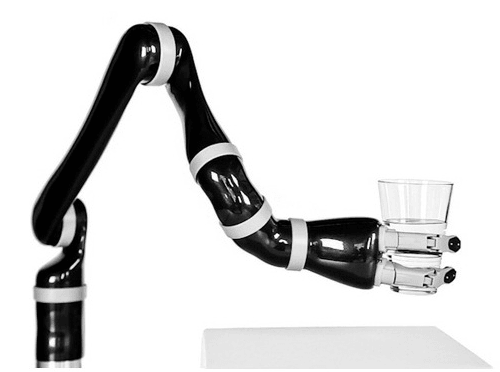
\includegraphics[width=\columnwidth]{img/jaco.png}
	\caption{Robotska ruka Jaco.\protect\footnotemark}
	\label{fig:jaco}
\end{figure}
\footnotetext{Preuzeto sa \url{https://smashingrobotics.com}}

\section{Problem dohvaćanja objekta}

Robotska ruka može izvršavati niz zadataka, poput dohvaćanja predmeta u prostoru, prijenosa tog istog objekta, rotiranja objekta, izbjegavanja različitih prepreka i sl. U ovom diplomskog radu ću rješavati problem dohvaćanja predmeta u prostoru, prvo bez prepreka, a nakon toga uz izbjegavanja prepreka u prostoru. Cilj problema je krajnjim efektorom robotske ruke doći do određenog objekta u prostoru.

Kako bismo povezali problem inverzne kinematike uz pomoć dubokog potpornog učenja, moramo napraviti neke poveznice. Okruženje u kojem će agent djelovati, očito će biti okruženje robota. Opservacija prostora će se sastojati od položaja vrha robotske ruke i položaja predmeta. U problemu s preprekama, opservacija će još sadržavati i položaje prepreka te položaje ostalih zglobova robotske ruke. Prostor akcija će biti šest brzina koje će se rasporediti na zglobove ruke. Ono što predstavlja glavni dio istraživanja ovog diplomskog rada je uspoređivanje različitih nagrada, odnosno funkcija gubitka. 

\section{Implementacija manipulatora u simulatoru}

Robotska ruka Jaco je ostvarena u simulatoru uz pomoć programskog jezika Python i niza njegovih biblioteka koje ću opisati u nastavku.

Fizički model je ostvaren uz pomoć biblioteke Bullet \citep{bullet}. Biblioteka je originalno napisana u C++, a oko te biblioteke napisan je omotač u Pythonu imena PyBullet koji omogućava korištenje Bulleta u Pythonu. No, PyBullet nije korišten direktno već uz biblioteku Pyb-Manipulator koja simulira različite manipulatore uz pomoć PyBulleta. Jedan od manipulatora koji je ostvaren u toj biblioteci je i robotska ruka Jaco koju koristim u ovom diplomskom radu.

Algoritmi dubokog potpornog učenja su ostvareni pomoću biblioteke OpenAI Gym \citep{gym}. Biblioteka omogućava jednostavno uključivanje fizikalni simulacija u okruženja dubokog potpornog učenja te testiranje i uspoređivanje različitih algoritama. Implementacije algoritama, konkretno algoritma proksimalne optimizacije politike, su ostvarene pomoću biblioteke OpenAI Baselines \citep{baselines} koja sadrži implementacije raznih algoritama dubokog potpornog učenja. Algoritmi su optimizirani i testirani te spremni za korištenje u istraživanjima.

Konačno, sve ovo je trebalo povezati u okruženje za treniranje. Okruženje treba stvoriti robotsku ruku Jaco, inicijalizirati okruženje ruke, inicijalizirati ciljni predmet koji je ostvaren u obliku male kuglice na slučajnu lokaciju u prostoru, inicijalizirati prepreke koje su ostvarene u obliku tri kugle na slučajne lokacije u prostoru te definirati funkcije koje će agent koristiti. Potrebno je bilo definirati funkciju korak (engl.~\emph{step}) koja će primiti akciju od agenta, provesti tu akciju u okruženju, izračunati gubitak i vratiti ga nazad agentu. Također, funkcija mora vraćati jesmo li došli do kraja epizode. Kraj epizode je definiran ako je robot došao do cilja ili je robot udario u prepreku. Potrebno je bilo i definirati funkciju resetiranja (engl.~\emph{reset}) koja će ponovo inicijalizirati ruku, okruženje, cilj i prepreke. Najbitnija stvar ovog diplomskog rada, a i svakog problema dubokog potpornog učenja je pronaći odgovarajuću nagradu, odnosno funkciju gubitka. 


\begin{figure}[ht!]
	\centering
	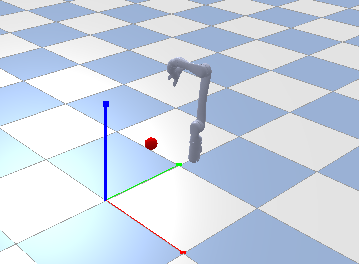
\includegraphics[width=\columnwidth]{img/bezprepreka.png}
	\caption{Problem bez prepreka.}
	\label{fig:bezprepeka}
\end{figure}

\begin{figure}[ht!]
	\centering
	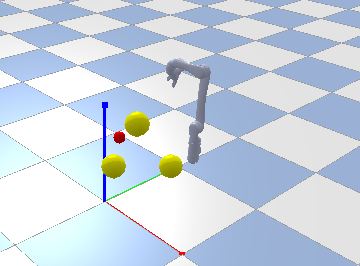
\includegraphics[width=\columnwidth]{img/spreprekama.png}
	\caption{Problem s preprekama.}
	\label{fig:sprepekama}
\end{figure}


\clearpage
\chapter{Rezultati}
\section{Izlaz agenta}

Agent tijekom učenja izbacuje varijable koje nam mogu pomoći da vidimo koliko dobro agent izvršava zadatak. Izlaz algoritma se zapisuje u datoteku u formatu odvojenom zarezima (engl.~\emph{csv - comma separated values}) te na standardni izlaz. Na standardni izlaz se ispisuje u obliku kao u tablici \ref{tab:izlaz_agenta}.

\begin{table}[ht!]
\centering
\caption{Izlaz agenta}
\label{tab:izlaz_agenta}
\begin{tabular}{@{}ll@{}}
\hline
Ime parametra   & Vrijednost \\
\hline
\hline
 eplenmean               & 5e+03       \\
 eprewmean               & -5.09e+03   \\
 fps                     & 5.54e+03    \\
 loss/approxkl           & 0.0064      \\
 loss/clipfrac           & 0.0686      \\
 loss/policy\_entropy     & 8.43       \\
 loss/policy\_loss        & -0.0045    \\
 loss/value\_loss         & 104        \\
 misc/explained\_variance & 0.00614    \\
 misc/nupdates          & 3           \\
 misc/serial\_timesteps   & 6.14e+03   \\
 misc/time\_elapsed       & 141        \\
 misc/total\_timesteps    & 7.86e+05   \\
\hline 
\end{tabular}
\end{table}

Duljina epizode (engl.~\emph{eplenmean}) nam govori koliko dugo je trebalo ruci da dosegne lopticu. Maksimalan broj koraka koji agent može napraviti unutar jedne epizode je 5000. Ovaj limit je postavljen da epizoda ne bi trajala beskonačno jer ako ruka nije unutar 5000 koraka dohvatila lopticu, vjerojatno neće nikada. Ovo je najbitniji parametar jer nam govori koliko dobro algoritam radi stvarni zadatak koji smo mu zadali. Što je ovaj broj manji, algoritam je bolji.

Prosječna nagrada u epizodi (engl.~\emph{eprewmean}) nam govori kolika je prosječna nagrada u epizodi. Agent u svakom koraku dobije nagradu, odnosnu gubitak za taj korak, a ovo je samo suma tih gubitaka kroz čitavu epizodu. Ovaj parametar je također bitan i govori nam kako radi algoritam, no ovisi o funkciji gubitka koju smo zadali tako da je nemoguće uspoređivati razne funkcije gubitka po ovom parametru. No, ako primijetimo da ova funkcija pada tijekom treniranja, znači da algoritam ide u dobrom smjeru.

Broj koraka u sekundi (engl.~\emph{fps - frame per second}) označava brzinu treniranja na našem računalu. Kullback-Leiblerov (engl.~\emph{loss/approxkl}) gubitak nam govori koliko se brzo politika trenutno mijenja. Postotak odsjecanja (engl.~\emph{loss/clipfrac}) nam govori koliko često je gradijent bio odsjecan. Entropija politike (engl.~\emph{loss/policy\_entropy}) nam govori koliko je politika slučajna, ovaj broj treba padati tijekom treniranja. Gubitak politike (engl.~\emph{loss/policy\_loss}) nam govori kolika je vrijednost gradijenta funkcije politike. Gubitak vrijednosti (engl.~\emph{loss/value\_loss}) nam govori kolika je vrijednost gradijenta funkcije vrijednosti.

Objašnjena varijanca (engl.~\emph{misc/explained\_variance}) nam govori koliko dobro funkcija vrijednosti objašnjava vraćenu vrijednost. Broj ažuriranja (engl.~\emph{misc/nupdates}) nam govori koliko puta smo ažurirali parametre politike i funkcije vrijednosti. 

Broj serijskih koraka(engl.~\emph{misc/serial\_timesteps}) i broj ukupnih koraka (engl.~\emph{misc/total\_timesteps}) nam govori koliko serijskih, odnosno ukupno koraka je napravljeno. Agenta treniramo paralelno, na više okruženja odjednom (točnije 128), pa broj serijskih koraka govori koliko koraka je napravljeno u pojedinom okruženju, a broj ukupnih koraka govori koliko koraka je napravljeno u svim okruženjima. Proteklo vrijeme (engl.~\emph{misc/time\_elapsed}) nam govori koliko je proteklo vremena u sekundama.

Za uspoređivanje različitih funkcija gubitka koristit ćemo tri parametra, trajanje epizode, prosječnu nagradu u epizodi i ukupan broj koraka.


Kod svih robotskih zadataka, potrebno je kažnjavati brzinu kojom se robot kreće s ciljem da se robot ili robotska ruka giba što moguće nježnije te bez naglih pokreta zbog sigurnosti. Brzinu ćemo kažnjavati kao negativnu normu vektora brzine koji sadrži brzine zglobova. 

\section{Rezultati problema bez prepreka}

Kod problema bez prepreka jedine stvari za koje imamo informaciju u prostoru su pozicija cilja i pozicija vrha ruke. Stvar koja nam se nameće da kažnjavamo je udaljenost između te dvije pozicije, naravno kao negativnu normu vektora udaljenosti. Ono što također možemo raditi je da nagrađujemo agenta ako je napredovao u odnosu na protekli korak. Dakle, pamtimo normu udaljenosti iz prethodnog koraka i nagrađujemo agenta ako je bolji nego prije. Iz ovoga imamo tri funkcije gubitka, prva je udaljenost i brzina, druga napredak i brzina, a treća udaljenost, napredak i brzina. Sve vrijednosti su skalirane da budu otprilike u jednakoj skali te ćemo sve funkcije gubitka trenirati na 20 milijuna koraka.

\begin{lstlisting}[caption={Kod za udaljenost i brzinu},language=Python]
observation = self.get_observation()
distance_vector = observation[:3] - self.target
distance_reward = - np.linalg.norm(distance_vector)
speed_reward = - np.linalg.norm(action)
reward = distance_reward + speed_reward
\end{lstlisting}

\begin{table}[ht!]
\centering
\caption{Rezultati za udaljenost i brzinu}
\label{tab:rub}
\begin{tabular}{@{}lll@{}}
\hline
eplenmean & eprewmean & misc/total\_timesteps \\
\hline
\hline
5001.00 & -4644.67 & 1.57e+06 \\ 
5001.00 & -4405.25 & 2.88e+06 \\ 
4934.95 & -4400.78 & 4.19e+06 \\ 
5001.00 & -4487.64 & 5.51e+06 \\ 
4976.26 & -4392.46 & 6.82e+06 \\ 
4860.11 & -4157.88 & 8.13e+06 \\ 
4916.93 & -4253.58 & 9.44e+06 \\ 
4879.62 & -4589.74 & 1.07e+07 \\ 
4953.33 & -4476.76 & 1.21e+07 \\ 
4911.33 & -4511.79 & 1.34e+07 \\ 
4862.73 & -4430.52 & 1.47e+07 \\ 
4928.81 & -4643.92 & 1.60e+07 \\ 
4973.91 & -4636.84 & 1.73e+07 \\ 
5001.00 & -4764.21 & 1.86e+07 \\ 
4968.79 & -4585.88 & 1.99e+07 \\ 
\hline
\end{tabular}
\end{table}

Iz tablice \ref{tab:rub} možemo vidjeti da prosječno trajanje epizode i prosječna nagrada se ne smanjuju kako vrijeme prolazi te ova funkcija gubitka nije dobra za ovaj problem. Ruka u rijetkim trenutcima dosegne cilj.


\begin{lstlisting}[caption={Kod za napredak i brzina},language=Python]
observation = self.get_observation()
distance_vector = observation[:3] - self.target
distance_reward = - np.linalg.norm(distance_vector)
progress_reward = - 300 * (-distance_reward +
		self.distance_reward_old)
self.distance_reward_old = distance_reward
speed_reward = - np.linalg.norm(action)
reward = progress_reward + speed_reward
\end{lstlisting}

\begin{table}[ht!]
\centering
\caption{Rezultati za napredak i brzinu}
\label{tab:rnb}
\begin{tabular}{@{}lll@{}}
\hline
eplenmean & eprewmean & misc/total\_timesteps \\
\hline
\hline
4558.74 & -2145.22 & 1.57e+06 \\ 
3990.53 & -1814.93 & 2.88e+06 \\ 
1933.10 & -884.44 & 4.19e+06 \\ 
1260.32 & -582.99 & 5.51e+06 \\ 
1300.25 & -597.80 & 6.82e+06 \\ 
1016.17 & -468.28 & 8.13e+06 \\ 
885.16 & -409.56 & 9.44e+06 \\ 
824.18 & -381.70 & 1.07e+07 \\ 
928.05 & -428.19 & 1.21e+07 \\ 
890.89 & -412.20 & 1.34e+07 \\ 
793.56 & -358.08 & 1.47e+07 \\ 
854.25 & -394.39 & 1.60e+07 \\ 
711.99 & -326.41 & 1.73e+07 \\ 
746.49 & -337.91 & 1.86e+07 \\ 
791.45 & -361.71 & 1.99e+07 \\ 
\hline
\end{tabular}
\end{table}

Iz tablice \ref{tab:rnb} vidimo da u odnosu na udaljenost i brzinu, ovdje vidimo značajan napredak. Ruka uspije pronaći cilj u otprilike 800 koraka i skoro svaki put, gubitak se smanjio tijekom treniranja i konvergirao na otprilike -350. Ova funkcija uspješno rješava problem dohvaćanja cilja s rukom.

\begin{lstlisting}[caption={Kod za udaljenost, napredak i brzina},language=Python]
observation = self.get_observation()
distance_vector = observation[:3] - self.target
distance_reward = - np.linalg.norm(distance_vector)
progress_reward = - 300 * (-distance_reward +
		self.distance_reward_old)
self.distance_reward_old = distance_reward
speed_reward = - np.linalg.norm(action)
reward = distance_reward + progress_reward + speed_reward
\end{lstlisting}

\begin{table}[ht!]
\centering
\caption{Rezultati za udaljenost, napredak i brzinu}
\label{tab:runb}
\begin{tabular}{@{}lll@{}}
\hline
eplenmean & eprewmean & misc/total\_timesteps \\
\hline
\hline
3819.96 & -3031.81 & 1.57e+06 \\ 
3578.17 & -2906.71 & 2.88e+06 \\ 
2264.80 & -1710.63 & 4.19e+06 \\ 
1791.30 & -1360.40 & 5.51e+06 \\ 
1497.91 & -1119.63 & 6.82e+06 \\ 
1110.11 & -774.56 & 8.13e+06 \\ 
971.30 & -714.09 & 9.44e+06 \\ 
977.26 & -753.41 & 1.07e+07 \\ 
1102.77 & -832.46 & 1.21e+07 \\ 
830.59 & -669.11 & 1.34e+07 \\ 
779.17 & -604.76 & 1.47e+07 \\ 
773.30 & -599.63 & 1.60e+07 \\ 
807.47 & -645.58 & 1.73e+07 \\ 
719.24 & -580.12 & 1.86e+07 \\ 
701.33 & -577.36 & 1.99e+07 \\ 
\hline
\end{tabular}
\end{table}

Iz tablice \ref{tab:runb} vidimo da ova funkcija gubitka također uspješno rješava problem, na kraju treniranja prosječno vrijeme epizode je nešto manje nego za prethodnu funkciju, funkcija gubitka je veća, no to je zbog toga što ova funkcija gubitka kažnjava i udaljenost pa nije moguće uspoređivati te dvije funkcije. Zaključujemo da je ova funkcija najbolja za dani problem jer ga rješava skoro svaki put i u najmanjem broju koraka.


\section{Rezultati problema s preprekama}

Problem s preprekama je izuzetno kompliciraniji nego problem bez prepreka. Odjednom više ruka ne može se jednostavno u svakom koraku samo približavati cilju jer se između nje i cilja može nalaziti prepreka. Ruka treba pronalaziti putanju između prepreka koju ponekad možda bude i nemoguće pronaći. 

Prva funkcija gubitka koju smo pokušali je linearno kažnjavala blizinu do najbliže prepreke. Ako je udaljenost do najbliže prepreke velika, kazna je jako mala, a ako je udaljenost mala, kazna je također velika. Ako bi ruka udarila u prepreku, epizoda je završila. Također, ako bi došao do cilja jednokratno bi bio jako nagrađen, a ako je udario u prepreku jednokratno bi bio jako kažnjen.

\begin{lstlisting}[caption={Kod za linearno kažnjavanje blizine i fiksne nagrade na kraju epizode},language=Python]

#reward calculation
observation = self.get_observation()
distance_vector = observation[:3] - self.target
distance_reward = - np.linalg.norm(distance_vector)
progress_reward = - 300 * (-distance_reward +
		self.distance_reward_old)
self.distance_reward_old = distance_reward
speed_reward = - np.linalg.norm(action)
min_obstacle_distances = self.min_obstacle_distances()
obstacle_reward = -0.4/np.min(min_obstacle_distances)+1.2
reward = distance_reward + progress_reward +
		speed_reward + obstacle_reward

# check if the goal has been reached
# otherwise check if the episode is over
if np.linalg.norm(distance_vector) < 0.05:
    reward = 2000
    done = True
elif np.any(min_obstacle_distances < 0.15):
    reward = -1000
    done = True
elif self.numberOfSteps > self.episodeLength:
    done = True
else:
    done = False
\end{lstlisting}

\begin{table}[ht!]
\centering
\caption{Rezultati za linearno kažnjavanje blizine prepreke i fiksne nagrade na kraju epizode}
\label{tab:rlk}
\begin{tabular}{@{}lll@{}}
\hline
eplenmean & eprewmean & misc/total\_timesteps \\
\hline
\hline
4660.64 & -4230.35 & 1.57e+06 \\ 
4067.72 & -3506.76 & 2.88e+06 \\ 
3041.90 & -2856.47 & 4.19e+06 \\ 
3681.57 & -3091.60 & 5.51e+06 \\ 
3496.40 & -3116.02 & 6.82e+06 \\ 
3568.77 & -3106.93 & 8.13e+06 \\ 
3296.14 & -2790.05 & 9.44e+06 \\ 
3704.81 & -2935.27 & 1.07e+07 \\ 
3625.26 & -3061.75 & 1.21e+07 \\ 
3196.91 & -2385.26 & 1.34e+07 \\ 
2445.88 & -1936.88 & 1.47e+07 \\ 
2597.89 & -1847.29 & 1.60e+07 \\ 
2053.09 & -1335.68 & 1.73e+07 \\ 
1389.56 & -628.74 & 1.86e+07 \\ 
1786.80 & -1134.73 & 1.99e+07 \\ 
\hline
\end{tabular}
\end{table}

\vspace{10pt}

Iako rezultati iz tablice \ref{tab:rlk} izgledaju dobro, oni su u stvarnosti jako loši. Rezultate u stvarnosti gledamo tako da pokrenemo naučenog agenta u okruženju i sami vizualno gledamo što se događa. Ono što je agent naučio s ovom funkcijom gubitka je to da mu se najbolje odmah zabiti u prvu prepreku, kazna će mu biti mala jer epizoda neće trajati dugo i sastojat će se većinom od fiksne kazne udaranja u prepreku. 

Ovo očito nije bilo rješenje našeg problema. Zbog toga smo pokušali izmijeniti funkciju gubitka tako da epizoda nije završavala prilikom udaranja u prepreku. Kad bi se ruka nalazila u blizini prepreke ili udarila u prepreku, samo bi imala veliki gubitak zbog gubitka blizine prepreke. Također, fiksne nagrade su ukinute. Naravno, kad nakon treniranja pokrećemo agenta da vidimo kako radi, ako on udari u prepreku, završit ćemo epizodu.

\begin{lstlisting}[caption={Kod za linearno kažnjavanje blizine i bez završavanja prilikom udarca u prepreku},language=Python]
observation = self.get_observation()
distance_vector = observation[:3] - self.target
distance_reward = - np.linalg.norm(distance_vector)
progress_reward = - 300 * (-distance_reward +
		self.distance_reward_old)
self.distance_reward_old = distance_reward
speed_reward = - np.linalg.norm(action)
min_obstacle_distances = self.min_obstacle_distances()
obstacle_reward = -0.4/np.min(min_obstacle_distances)+1.2
reward = distance_reward + progress_reward +
		speed_reward + obstacle_reward
# check if the goal has been reached or episode over
if np.linalg.norm(distance_vector) < 0.05:
    done = True
elif np.any(min_obstacle_distances < 0.15):
    done = False
elif self.numberOfSteps > self.episodeLength:
    done = True
else:
    done = False
\end{lstlisting}

\begin{table}[ht!]
\centering
\caption{Rezultati za linearno kažnjavanje blizine i bez završavanja prilikom udarca u prepreku}
\label{tab:rbk}
\begin{tabular}{@{}lll@{}}
\hline
eplenmean & eprewmean & misc/total\_timesteps \\
\hline
\hline
4853.53 & -9865.14 & 1.57e+06 \\ 
4960.64 & -10915.79 & 2.88e+06 \\
4919.95 & -9538.70 & 4.19e+06 \\ 
4625.72 & -8614.35 & 5.51e+06 \\ 
4683.32 & -9372.60 & 6.82e+06 \\ 
4557.16 & -8919.95 & 8.13e+06 \\ 
4165.51 & -7997.34 & 9.44e+06 \\ 
4299.81 & -8486.60 & 1.07e+07 \\ 
4245.40 & -8459.33 & 1.21e+07 \\ 
3756.71 & -7258.29 & 1.34e+07 \\ 
4494.71 & -8596.00 & 1.47e+07 \\ 
4400.12 & -7979.35 & 1.60e+07 \\ 
4069.01 & -7443.17 & 1.73e+07 \\ 
4042.78 & -7213.07 & 1.86e+07 \\ 
3930.52 & -7177.77 & 1.99e+07 \\ 
\hline
\end{tabular}
\end{table}

Iz tablice  \ref{tab:rbk} vidimo da novi rezultati izgledaju lošije nego prethodni, no u stvarnosti su bolji. Agent izbjegava prepreke, te u nekim slučajevima pronađe put do cilja. Problematičan mu je slučaj kad mu je cilj skriven iza prepreke. Prepreka ga odbija isto onoliko koliko ga cilj privlači te agent u tom slučaju najčešće samo stoji u mjestu.

Pokušat ćemo eksponencijalno kažnjavati blizinu prepreke te dvostruko više nagrađivati približavanje cilju. Ovo bi za posljedicu trebalo imati da algoritam zaobilazi prepreke u kružnom luku i tako lakše dolazi do cilja.

\begin{lstlisting}[caption={Kod za eksponencijalno kažnjavanje blizine i bez završavanja prilikom udarca u prepreku},language=Python]
observation = self.get_observation()
distance_vector = observation[:3] - self.target
distance_reward = - np.linalg.norm(distance_vector)
progress_reward = - 2 * 300 * (-distance_reward +
		self.distance_reward_old)
self.distance_reward_old = distance_reward
speed_reward = - np.linalg.norm(action)
min_obstacle_distances = self.min_obstacle_distances()
obstacle_reward = -0.02/(np.min(min_obstacle_distances)**3)
reward = distance_reward + progress_reward +
		speed_reward + obstacle_reward
# check if the goal has been reached
# otherwise check if the episode is over
if np.linalg.norm(distance_vector) < 0.05:
    done = True
elif np.any(min_obstacle_distances < 0.15):
    done = False
elif self.numberOfSteps > self.episodeLength:
    done = True
else:
    done = False
\end{lstlisting}

\begin{table}[ht!]
\centering
\caption{Rezultati za eksponencijalno kažnjavanje blizine i bez završavanja prilikom udarca u prepreku}
\label{tab:rek}
\begin{tabular}{@{}lll@{}}
\hline
eplenmean & eprewmean & misc/total\_timesteps \\
\hline
\hline
4877.34 & -11253.18 & 1.57e+06 \\ 
4679.16 & -10129.53 & 2.88e+06 \\ 
4122.46 & -9429.34 & 4.19e+06 \\ 
3730.75 & -8085.56 & 5.51e+06 \\ 
4014.43 & -7986.74 & 6.82e+06 \\ 
3106.13 & -6309.29 & 8.13e+06 \\ 
3120.73 & -6476.75 & 9.44e+06 \\ 
1998.13 & -3773.81 & 1.07e+07 \\ 
1702.80 & -2987.62 & 1.21e+07 \\ 
2300.74 & -4048.41 & 1.34e+07 \\ 
2318.29 & -4525.41 & 1.47e+07 \\ 
1770.62 & -3393.89 & 1.60e+07 \\ 
2229.36 & -4106.26 & 1.73e+07 \\ 
1683.42 & -3848.00 & 1.86e+07 \\ 
1239.36 & -2636.43 & 1.99e+07 \\ 
\hline
\end{tabular}
\end{table}


Iz tablice \ref{tab:rek} vidimo da se ova funkcija gubitka ponaša upravo onako kako smo željeli. Odlično rješava naš problem i agent uspješno zaobilazi prepreke. No, stvar koju možemo primijetiti da agent nije konvergirao za 20 milijuna koraka te ćemo ga pustiti da se trenira na 40 milijuna koraka. 

\begin{table}[ht!]
\centering
\caption{Rezultati za eksponencijalno kažnjavanje blizine i bez završavanja prilikom udarca u prepreku na 40 milijuna koraka}
\label{tab:cetm}
\begin{tabular}{@{}lll@{}}
\hline
eplenmean & eprewmean & misc/total\_timesteps \\
\hline
\hline
4661.85 & -9838.50 & 2.88e+06 \\ 
4137.11 & -8440.07 & 5.51e+06 \\ 
3791.15 & -7692.32 & 8.13e+06 \\ 
2962.36 & -5753.18 & 1.07e+07 \\ 
2715.98 & -5039.09 & 1.34e+07 \\ 
2221.33 & -4388.06 & 1.60e+07 \\ 
1667.47 & -3272.12 & 1.86e+07 \\ 
1704.15 & -3254.69 & 2.12e+07 \\ 
1323.04 & -2676.78 & 2.39e+07 \\ 
1401.51 & -2744.61 & 2.65e+07 \\ 
1364.24 & -2430.31 & 2.91e+07 \\ 
1106.77 & -2208.91 & 3.17e+07 \\ 
1154.20 & -2399.01 & 3.43e+07 \\ 
1256.99 & -2446.23 & 3.70e+07 \\ 
1100.65 & -2358.74 & 3.96e+07 \\ 
\hline
\end{tabular}
\end{table}

\vspace{100pt}

Iz tablice \ref{tab:cetm} vidimo da za 40 milijuna koraka agent konvergira te se iznimno dobro ponaša pri zaobilaženju prepreka. Naravno, u nekim konfiguracijama prostora ruka udari u prepreku jer zbog svojih fizikalnih ograničenja ne može dohvatiti cilj. Zaključujemo da je ova funkcija najbolja za dani problem od svih koje smo probali jer rješava problem skoro svaki put.

Nakon rješavanja problema dohvata cilja uz prepreke, proširili smo ograničenje da agent osim vrhom ruka, nijednim svojim dijelom ne smije udariti u prepreku. Kažnjavali smo eksponencijalno najbližu blizinu nekog zgloba do njemu najbliže prepreke.


\begin{table}[ht!]
\centering
\caption{Rezultati za blizinu bilo kojeg dijela robota do prepreke}
\label{tab:svi}
\begin{tabular}{@{}lll@{}}
\hline
eplenmean & eprewmean & misc/total\_timesteps \\
\hline
\hline
4887.21 & -16079.80 & 2.88e+06 \\ 
4490.02 & -12362.30 & 5.51e+06 \\ 
4715.55 & -17295.69 & 8.13e+06 \\ 
4389.97 & -14387.87 & 1.07e+07 \\ 
3545.18 & -10016.69 & 1.34e+07 \\ 
3276.90 & -10959.46 & 1.60e+07 \\ 
2771.84 & -7745.69 & 1.86e+07 \\ 
2524.67 & -8585.83 & 2.12e+07 \\ 
2393.39 & -7386.62 & 2.39e+07 \\ 
2620.81 & -8626.77 & 2.65e+07 \\ 
2077.17 & -6748.79 & 2.91e+07 \\ 
2084.14 & -7185.85 & 3.17e+07 \\ 
1545.79 & -5538.39 & 3.43e+07 \\ 
1880.94 & -6492.34 & 3.70e+07 \\ 
1663.24 & -5263.44 & 3.96e+07 \\ 
\hline
\end{tabular}
\end{table} 

Iz tablice \ref{tab:svi} vidimo da ovi rezultati izgledaju dobro, no ipak se lošije ponaša nego kad smo gledali da samo vrh ruke ne smije udariti u prepreku. Razlog ovome što funkcija gubitka odjednom postaje još kompleksnija nego prije, agentu je teško procijeniti koji zglob je bitniji da se udalji o prepreke te na kraju pozicije svakog od zgloba su u nekoj mjeri ovisne jedna o drugoj.

\clearpage
\chapter{Zaključak}

Problem inverzne kinematike manipulatora riješili smo pomoću dubokog potpornog učenja. Robotska ruka je dobila svoj mozak i ponaša se inteligentno u zadatku dohvaćanja cilja u prostoru. Problem bez prepreka je uspješno riješen, ali apsolutno svakome je jasno da je ruka samo trebala skužiti da se u svakom trenutku samo mora približavati cilju. Problem s preprekama je donekle riješen, ruka ne uspije uvijek dohvatiti cilj, ali u većini slučajeva ga ipak dohvati. Ovaj problem je prilično složeniji, jer ruka više ne može samo pohlepno ići prema cilju, već se u nekim trenutcima mora i udaljavati od cilja da bi ga uspješno dohvatila.

Možemo primijetiti da povećavanjem težine zadatka, ruci postaje teže riješiti problem. Ono što se ljudima može činiti samo malo otežavanje, algoritmima umjetne inteligencije predstavlja ogromno otežavanje. Proći će sigurno još vremena prije nego što uspijemo usavršiti algoritme da sigurno obavljaju poslove koje želimo da obavljaju. 

Ovaj rad i probleme koji su rješavani u njemu, sigurno će biti zanimljivo ponovno pokušati riješiti za nekoliko godina. Vrlo vjerojatno ćemo tada imati algoritme koje će raditi još bolje od ovoga, imat ćemo računalnu opremu na kojoj ćemo još brže trenirati te iste algoritme i problemi koje smo rješavali u ovom radu možda postanu trivijalni. Pojavit će se tada sigurno problemi koji će postati teški i za te algoritme jer ipak ljudska sposobnost postavljanja novih problema će uvijek biti veća od mogućnosti rješavanja istih.

Duboko potporno učenje je jedna od najperspektivnijih grana razvoja umjetne inteligencije. U drugoj polovici 20. stoljeća, kada je umjetna inteligencija uzela maha, jako mnogo se pričalo o takozvanoj "tehnološkoj singularnosti", točki u vremenu kada će računala poprimiti vlastitu svijest i postati ravnopravna ljudima. No ipak, kad su shvaćena ograničenja umjetne inteligencije, priča o tome je prestala.

No, u zadnjih desetak godina, kada je duboko učenje uzelo maha, pa tako i duboko potporno učenje, ova tema je ponovno postala aktualna. Ono što se točno dešava unutar same neuronske mreže i na koji način ona uspijeva zaključiti neke stvari, ljudski mozak nije u stanju razumjeti. Mišljenja smo da ako će nas išta dovesti do "tehnološke singularnosti", onda je to duboko potporno učenje. U tom trenutku, duboko potporno učenje neće spadati više u povijest čovječanstva, već u povijest bogova.



%%%%%%%%%%%%%%%%%%%%%%%
\bibliography{literatura}
\bibliographystyle{fer}

%%%%%%%%%%%%%%%%%%%%%%%%%%%%

\begin{sazetak}

	Inverzna kinematika manipulatora učenja iznimno je kompliciran problem. Cilj ovog rada je bio riješiti taj problem uz pomoć dubokog potpornog učenja. Napravljen je pregled područja dubokog potpornog učenja, iznesene su teoretske osnove, ključni pojmovi dubokog potpornog učenja te algoritmi gradijenta politike. Riješen je problem dohvaćanja objekta u prostoru korištenjem robotske ruke Jaco, prvo u prostoru bez prepreka, a zatim i s preprekama.

	\kljucnerijeci{potporno učenje, duboko učenje, duboko potporno učenje, robotika, Jaco}
\end{sazetak}

\newpage

%%%%%%%%%%%%%%%%%%%%%%%%%%%%%%%
\engtitle{Inverse kinematics of robotic manipulators achieved using deep reinforcement learning}
\begin{abstract}

Inverse kinematics of robotic manipulators is a very complicated problem. The aim of this thesis was to solve that problem using deep reinforcement learning. An overview of the area of deep reinforcement learning was made, the theoretical foundations, key concepts of deep supportive learning and policy gradient algorithms were presented. Problem of reaching target in space using robotic manipulator arm Jaco was solved, first in space without obstacles and then in space with obstacles.

	
	\keywords{reinforcement learning, deep learning, deep reinforcement learning, robotics, Jaco}

	%%%%%%%%%%%%%%%%%%%%5
\end{abstract}
\end{document}